
%\section*{Bloque F: Evaluación del programa de fidelización (márgenes intensivo vs. extensivo)}


% Serviclub es el programa de fidelización. LA APP no es Serviclub, sino una herramienta para usar Serviclub, en donde acumulás y canjeas puntos por descuentos, productos o beneficios. Existen Cliente Serviclub que NO usan la app, a YPF le conviene que usen la App porque le permite trackear mejor el consumo y habilita marketing personalizado.

\subsection{Motivación}
Los programas de fidelización no solo buscan retener clientes: también generan datos valiosos sobre comportamiento de consumo y respuesta a incentivos. Sin embargo, el hecho de que los socios consuman más que los no socios no implica que el programa cause ese mayor consumo. Puede simplemente reflejar que quienes más cargan nafta son también quienes más se afilian. El objetivo de esta propuesta es ir más allá de esa comparación descriptiva y estimar el efecto causal del programa sobre ventas, mix de productos y márgenes.
Para eso planteamos una batería de tres ejercicios complementarios, cada uno diseñado para aislar un aspecto distinto del impacto de Serviclub. Los tres pueden implementarse en conjunto y sus resultados se refuerzan mutuamente.

\subsection{Objetivos}
Las preguntas centrales que guían el análisis son:


\begin{itemize}
    \item ¿El programa aumenta la frecuencia de carga y consumo de sus socios, o solo los atrae porque ya cargaban más?
    \item ¿Qué tipo de beneficios generan mayor consumo adicional?
    \item ¿La variedad de productos que consumen difiere entre socios y no socios?
    \item ¿Los socios responden más a mejoras en la experiencia de la estación que los no socios?
    \item ¿La fidelización se explica por los beneficios del programa, o por la experiencia integral de compra?
    %\item ¿Qué campañas logran \emph{fidelizar} a los clientes?
\end{itemize}

\subsection{Diseño general}
El desafío metodológico principal es que la base de datos de \emph{Serviclub} registra el consumo una vez que el cliente ya es socio, pero no antes de su afiliación. Esto impide, en principio, comparar directamente el comportamiento de cada cliente antes y después de unirse al programa\footnote{En caso de que las bases de transacciones cuenten con datos de tarjetas de crédito/débito que permitan trackear clientes no-socios existirían más alternativas.}.
Sin embargo, la combinación de datos transaccionales, uso de beneficios e implementación de campañas permite diseñar tres ejercicios cuasi-experimentales que sortean esta limitación de maneras distintas y complementarias. 

\subsubsection*{Ejercicio 1: El efecto de canjear premios sobre el consumo posterior}
\textbf{Pregunta:} ¿Redimir una recompensa (canje de puntos, descuento, beneficio) aumenta la frecuencia de carga u otros consumos en los meses siguientes?

\textbf{Lógica del ejercicio:} Dentro del universo de socios, no todos canjean premios con la misma frecuencia ni en los mismos momentos. Esto genera variación natural que puede aprovecharse: si dos socios con patrones de consumo similares difieren en si canjearon o no un beneficio en determinado mes, podemos comparar su comportamiento posterior.

La estrategia consiste en usar cada evento de canje como un ``experimento natural'' y analizar si el consumo del cliente aumenta en los meses siguientes respecto a su propio historial previo y respecto a socios similares que no canjearon en ese período. Este tipo de análisis, conocido como estudio de eventos, permite aislar el efecto del canje del resto de los factores que afectan el consumo.

Existe evidencia en la literatura de marketing que indica que redimir premios refuerza el hábito de compra: el cliente que canjea recibe una señal concreta del valor del programa, lo que incrementa su compromiso con la marca. Este ejercicio permite testear si eso ocurre en \emph{Serviclub}.

\textbf{Datos necesarios:} Historial de transacciones por cliente con fechas, montos y tipo de producto; registro de canjes con fecha y tipo de beneficio.

\subsubsection*{Ejercicio 2: Campañas de afiliación como fuente de variación}
\textbf{Pregunta:} ¿Los clientes que se afilian al programa por una campaña específica muestran un comportamiento distinto —y más sostenido— que quienes se afilian de forma espontánea?

\textbf{Lógica del ejercicio:} YPF implementa campañas de afiliación en distintos momentos y regiones (por ejemplo, promociones vinculadas a eventos, como las del Mundial). Estos lanzamientos generan "olas" de nuevos socios que se afilian en un período acotado y por un motivo identificable, lo que los hace comparables entre sí y distinguibles de quienes se afilian por iniciativa propia en otros momentos.

La estrategia consiste en comparar la evolución del consumo de dos grupos: los clientes que se afiliaron durante una campaña específica y los que se afiliaron de forma más gradual y espontánea en períodos sin campaña activa, controlando por características observables como estación habitual, tipo de vehículo y nivel de consumo previo estimado.

Si los clientes captados por campaña muestran mayor retención y consumo sostenido, eso indica que la campaña no solo amplía la base de socios sino que atrae perfiles más comprometidos. Si, en cambio, su comportamiento decae rápidamente tras el fin de la campaña, sugiere que el vínculo fue oportunista y no generó fidelización real.

Este ejercicio responde directamente a una pregunta de negocio concreta: ¿vale la pena invertir en campañas de afiliación masiva, o es mejor apostar a la afiliación orgánica?

\textbf{Datos necesarios:} Registro de afiliaciones con fecha y canal (campaña específica vs. espontáneo); historial de consumo post-afiliación; datos de estación y vehículo cuando estén disponibles.


\subsubsection*{Ejercicio 3: Complementariedad entre \emph{Serviclub} y la experiencia en la estación}
\textbf{Pregunta:} ¿Los socios de \emph{Serviclub} responden más a las mejoras en la estación que los no socios? ¿O dicho de otro modo: ¿el programa y la experiencia física se potencian mutuamente?

\textbf{Lógica del ejercicio:} Las remodelaciones de estaciones al formato YPF Full 
representan un cambio significativo en la experiencia de compra ---infraestructura, 
servicios, atención--- sin que el funcionamiento de \emph{Serviclub} se modifique. 
Sin embargo, las estaciones que se remodelan probablemente no son elegidas al azar: 
YPF puede priorizar estaciones con mayor potencial de crecimiento, mejor ubicación o 
determinado perfil de clientes. Esto implica un problema de selección: socios y no 
socios en esas estaciones podrían ser distintos \emph{antes} de la remodelación, lo 
que contaminaría cualquier comparación simple entre estaciones Full y no Full \footnote{Este tema se abordará en profundidad en el módulo correspondiente a la implementación de FULL}.

La estrategia para sortear este problema es agregar la dimensión temporal, comparando 
el comportamiento de cada grupo antes y después de la remodelación dentro de una misma 
estación. Esta metodología ---conocida como \emph{Triple Diferencia}--- controla por 
todas las características fijas de cada estación y de cada cliente, y permite 
identificar el cambio en la brecha entre socios y no socios que ocurre justo cuando 
la estación se remodela, no el nivel absoluto de esa brecha.

En términos concretos, el modelo compara cuatro grupos simultáneamente (ver Cuadro \ref{tab:triple_diff}): socios y no socios, en estaciones Full y no Full, antes y después de la remodelación. El coeficiente clave mide si el efecto de la remodelación sobre el consumo es distinto para socios que para no socios: si la remodelación beneficia por igual a ambos grupos, el efecto se explica por la mejora general de la estación; pero si el aumento es significativamente mayor entre los socios, eso indica que el programa y la experiencia física se potencian mutuamente.

Si se encuentra esa complementariedad, las implicancias para la empresa son dobles.Por un lado, la inversión en remodelaciones Full genera un retorno adicional entre los clientes ya fidelizados por \emph{Serviclub}, lo que fortalece el caso para priorizar esas inversiones en estaciones con alta penetración del programa. Por otro lado, el programa estaría siendo subutilizado en estaciones no Full: los mismos incentivos rinden menos donde la experiencia de compra es de menor calidad. En conjunto, esto sugiere que la expansión de \emph{Serviclub} y la mejora de infraestructura son decisiones que conviene coordinar, y no evaluar de forma independiente.

\textbf{Datos necesarios:} Fechas de remodelación por estación; historial de transacciones distinguiendo socios y no socios; datos suficientes antes y después de cada remodelación para al menos un subconjunto de estaciones.



\begin{table}[h]

\centering
\caption{Estructura de la Triple Diferencia}
\label{tab:triple_diff}
\setlength{\extrarowheight}{4pt}
\begin{tabular}{lcc}
\hline\hline
 & \textbf{Antes de remodelación} & \textbf{Después de remodelación} \\
\hline
\textit{Estación Full} & & \\
\quad Socio Serviclub   & $A$ & $B$ \\
\quad No socio          & $C$ & $D$ \\[4pt]
\textit{Estación no Full} & & \\
\quad Socio Serviclub   & $E$ & $F$ \\
\quad No socio          & $G$ & $H$ \\
\hline\hline
\multicolumn{3}{p{10cm}}{\footnotesize El efecto buscado es: 
$[(B-A)-(D-C)] - [(F-E)-(H-G)]$. 
Si este valor es positivo y significativo, existe complementariedad entre 
el programa \emph{Serviclub} y la experiencia en estaciones Full.}\\
\end{tabular}
\end{table}

\begin{table}[h]
\centering
\small
\setlength{\extrarowheight}{5pt}
\setlength{\tabcolsep}{10pt}
\begin{tabular}{lcccc}
\hline\hline
 & \multicolumn{2}{c}{\cellcolor{corporateblue!12}\textbf{Antes}}
 & \multicolumn{2}{c}{\cellcolor{corporateblue!38}\textbf{Después}} \\
 & \cellcolor{corporateblue!12}\small\textbf{Socio}
 & \cellcolor{corporategray!20}\small\textbf{No socio}
 & \cellcolor{corporateblue!12}\small\textbf{Socio}
 & \cellcolor{corporategray!20}\small\textbf{No socio} \\
\hline
\textit{Estación Full}
 & \cellcolor{corporateblue!22}$A$
 & \cellcolor{corporategray!12}$C$
 & \cellcolor{corporateblue!52}$B$
 & \cellcolor{corporategray!38}$D$ \\
\textit{Estación no Full}
 & \cellcolor{corporateblue!22}$E$
 & \cellcolor{corporategray!12}$G$
 & \cellcolor{corporateblue!52}$F$
 & \cellcolor{corporategray!38}$H$ \\
\hline\hline
\end{tabular}

\vspace{0.6em}
\[
\text{Efecto buscado} =
\underbrace{(B - A) - (D - C)}_{\text{DiD en estaciones Full}}
\;-\;
\underbrace{(F - E) - (H - G)}_{\text{DiD en estaciones no Full}}
\]
{\footnotesize\color{corporategray}\itshape
Tonos más oscuros = período post-remodelación.\quad
Azul: socios \emph{Serviclub}.\quad Gris: no socios.}
\end{table}

\begin{figure}
    \centering
    \caption{Diagrama ilustrativo de la Triple Diferencia}
    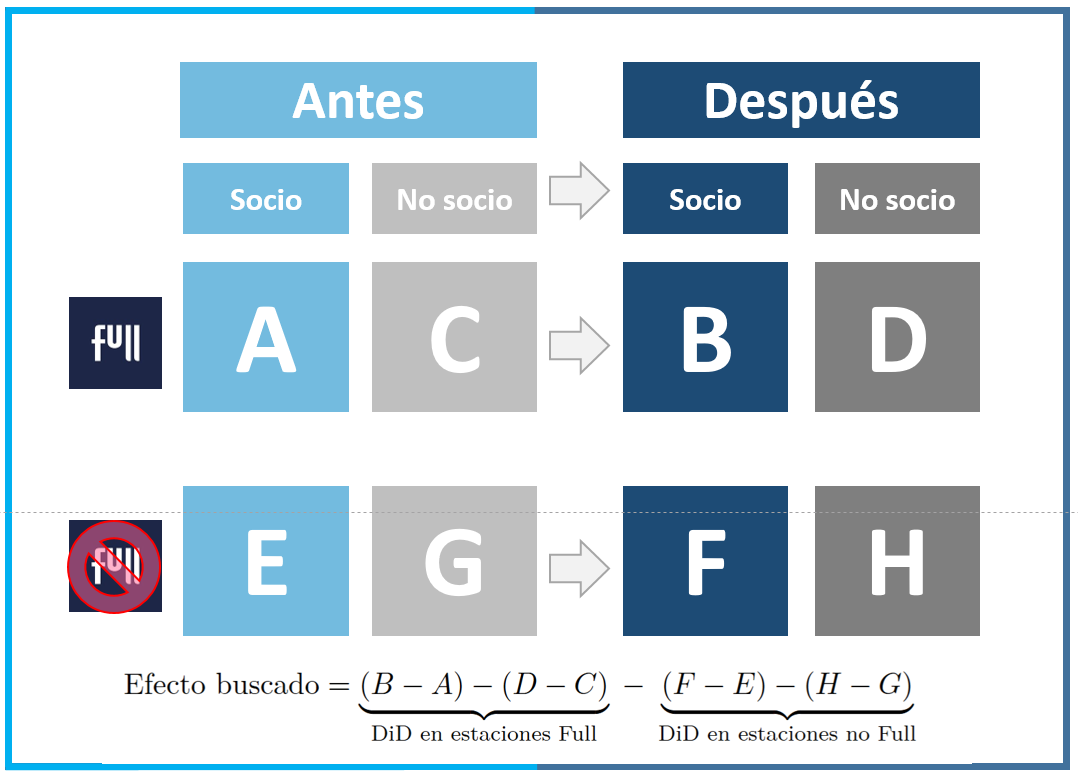
\includegraphics[width=0.6\textwidth]{../../imagenes/esquema_ddd.png}
\end{figure}



\textbf{Modelo base (triple diferencia):}
\[
y_{ist}=\beta_1 Socio_i + \beta_2 Full_{st} + \beta_3(Socio_i\times Full_{st}) + \alpha_i + \gamma_t + \delta_s + \varepsilon_{ist}
\]

donde $y_{ist}$ es el consumo de combustible del cliente $i$ en la estación $s$ y periodo $t$, $Socio_i$ es una variable indicadora de si el cliente es socio de \emph{Serviclub}, $Full_{st}$ indica si la estación $s$ fue remodelada al formato Full en el periodo $t$, $\alpha_i$ son efectos fijos de cliente, $\gamma_t$ efectos fijos de tiempo y $\delta_s$ efectos fijos de estación. Por lo que $\beta_3>0$ sugeriría que \emph{Serviclub} rinde mas donde mejora la experiencia integral.

\subsubsection*{Ejercicios adicionales}
\textcolor{red}{¿Qué campañas o beneficios fidelizan más? Event Study de campañas específicas}


\subsection{Datos requeridos}
Principales bases de datos y variables necesarias para este módulo:
\begin{itemize}
    \item Transacciones de estaciones de servicio: fecha, estación, litros, ticket, tipo de combustible, compras en tienda, método de pago, uso de la App, etc.
    \item Transacciones de clientes \emph{Serviclub}: IDEM anterior pero con identificación de \textbf{Cliente}, para poder construir panel individual.
    \item Información del cliente \emph{Serviclub}: \textbf{Cliente}, fecha de alta, edad, genero, localidad, etc.
    \item Canjes de clientes \emph{Serviclub}: \textbf{Cliente}, fecha, tipo de canje, puntos utilizados, beneficios obtenidos, exposición a campañas, etc.
\end{itemize}

El universo de análisis se definirá más adelante al conocer con más precisión la implementación del programa y campañas. Idealmente abarcaría varios meses o años, para poder observar la evolución del comportamiento de consumo antes y después de la afiliación al programa, así como la respuesta a diferentes campañas e incentivos. Además, será necesario contar con información detallada sobre promociones específicas y campañas ofrecidas dentro del programa, incluyendo fechas de implementación y alcance geográfico de las mismas.


\textbf{Minimo viable:}
\begin{itemize}
    \item panel transaccional de socios (fecha, estacion, litros, ticket, tipo de combustible, compras en tienda);
    \item fechas de alta, uso de App, canjes y exposicion a campanas;
    \item panel mensual por estacion (ventas totales, share \emph{Serviclub}, mix de productos, precios);
    \item calendario de campanas e implementaciones por zona/estacion;
    \item identificacion de remodelaciones Full para el ejercicio de complementariedad.
\end{itemize}


